\chapter{Mengukur Massa}\label{ch:g3:measuring-mass}

Di pasar: ``Apelnya sekilogram, ya!'' Penjualnya menuang apel ke dalam
piring \omterm{def:g3:levers-and-scales:scale}{neraca} sampai \omterm{def:g3:levers-and-scales:scale}{neracanya} puas. Apa tepatnya yang dipesan pembeli
itu --- dan bagaimana \omterm{def:g3:levers-and-scales:scale}{neraca} tahu kapan harus berhenti? Dengan \omterm{def:g3:levers-and-scales:lever}{tuas}
dan \omterm{def:g3:levers-and-scales:scale}{neraca} di dalam kotak alat kita, kita siap \omterm{def:g2:measuring-length:measure}{mengukur} hal yang baru:
\omterm{def:g3:measuring-mass:mass}{massa}.

\section{Massa: seberapa banyak zatnya}

\begin{definition}[Massa]\label{def:g3:measuring-mass:mass}
Yang disebut \emph{massa}\index{massa} sebuah benda menyatakan
seberapa banyak zat penyusunnya. Makin banyak zatnya, makin besar
massanya --- dan makin kuat Bumi menariknya ke bawah, itulah sebabnya
benda bermassa lebih besar terasa lebih berat di tanganmu dan menekan
piring \omterm{def:g3:levers-and-scales:scale}{neracanya} turun.
\end{definition}

\begin{example}[Besar bukan berarti berat]\label{ex:g3:measuring-mass:bignotcheavy}
Sebuah bantal memenuhi kedua lenganmu, namun kamu membawanya dengan
mudah. Sebuah batu yang lebih kecil daripada kepalan tanganmu membuat
pergelangan tanganmu tegang. Bantalnya besar tetapi berisi sedikit zat
--- kebanyakan bulu dan \omterm{def:g2:air-around-us:air}{udara}; batunya kecil tetapi padat berisi zat.
\omterm{def:g3:measuring-mass:mass}{Massa} berbicara tentang \emph{seberapa banyak zatnya}, bukan tentang
seberapa banyak ruang yang dipakainya. (Kedua gagasan ini, dan tarian
rumit di antara keduanya, akan bertemu lagi dalam kisah \omterm{def:g1:floating-and-sinking:words}{terapung} dan
\omterm{def:g1:floating-and-sinking:words}{tenggelam} suatu hari nanti.)
\end{example}

\begin{definition}[Gram dan kilogram]\label{def:g3:measuring-mass:units}
\omterm{def:g3:measuring-mass:mass}{Massa} diukur dalam \emph{gram}\index{gram} (ditulis \unit{g}) dan
\emph{kilogram}\index{kilogram} (ditulis \unit{kg}):
\[
\qty{1}{kg} = \qty{1000}{g}.
\]
Sebuah penjepit kertas bermassa kira-kira \qty{1}{g}; sebuah apel
kira-kira \qty{150}{g}; sekarton susu kira-kira \qty{1}{kg}; kamu
sendiri, beberapa puluh kilogram. Seperti \omterm{def:g2:measuring-length:units}{meter}, \omterm{def:g2:measuring-length:measure}{satuan} ini sama bagi
semua orang di Bumi.
\end{definition}

\section{Menimbang dengan neraca}

\begin{method}[Menimbang dengan balok]\label{met:g3:measuring-mass:weigh}
Untuk \omterm{def:g2:measuring-length:measure}{mengukur} \omterm{def:g3:measuring-mass:mass}{massa} sebuah melon dengan \omterm{def:g3:levers-and-scales:scale}{neraca} dan sekotak balok
logam bertanda (\qty{500}{g}, \qty{200}{g}, \qty{100}{g},
\qty{50}{g}, \dots):
\begin{enumerate}
  \item periksa bahwa \omterm{def:g3:levers-and-scales:scale}{neraca} kosongnya tergantung mendatar;
  \item letakkan melonnya di satu piring;
  \item tambahkan balok ke piring yang lain, mulai dari yang paling
        besar yang masih berguna, sampai kedua piring tergantung
        mendatar;
  \item jumlahkan baloknya: totalnya adalah \omterm{def:g3:measuring-mass:mass}{massa} melon itu.
\end{enumerate}
Kalau kedua piring mendatar dengan satu balok \qty{500}{g}, satu
\qty{200}{g}, dan satu \qty{100}{g}, \omterm{def:g3:measuring-mass:mass}{massa} melon itu $500 + 200 + 100 =
\qty{800}{g}$.
\end{method}

\begin{omfigure}
\begin{tikzpicture}[scale=0.85]
  \draw[thick] (5.5,0) -- (5.5,2.6);
  \draw[thick] (4.9,0) -- (6.1,0);
  \draw[very thick] (2.5,2.6) -- (8.5,2.6);
  \fill (5.5,2.6) circle (2.4pt);
  \draw[thick] (2.5,2.6) -- (2.2,1.5) (2.5,2.6) -- (2.8,1.5);
  \draw[thick] (1.9,1.5) .. controls (2.5,1.05) .. (3.1,1.5);
  \draw[thick] (8.5,2.6) -- (8.2,1.5) (8.5,2.6) -- (8.8,1.5);
  \draw[thick] (7.9,1.5) .. controls (8.5,1.05) .. (9.1,1.5);
  \draw[thick, fill=omMeth, fill opacity=0.4] (2.5,1.55) circle (0.42);
  \node[font=\footnotesize] at (2.5,1.55) {melon};
  % all three marked blocks, each with its value
  \draw[thick, fill=omExo, fill opacity=0.4] (8.0,1.2) rectangle (8.55,1.7);
  \node[font=\scriptsize] at (8.28,1.45) {$500$};
  \draw[thick, fill=omExo, fill opacity=0.4] (8.6,1.2) rectangle (8.95,1.5);
  \node[font=\scriptsize] at (8.78,1.35) {$200$};
  \draw[thick, fill=omExo, fill opacity=0.4] (8.1,1.7) rectangle (8.35,1.9);
  \node[font=\scriptsize] at (8.22,1.8) {$100$};
  \node[right, font=\footnotesize, align=left] at (9.35,1.7)
    {$500 + 200 + 100$:\\\qty{800}{g} balok};
  \node[below, font=\small] at (5.5,-0.3)
    {piring mendatar: massa melon sama dengan total baloknya};
\end{tikzpicture}

{\small Menimbang melon: balok ditambahkan sampai kedua piring
mendatar; jumlahnya adalah jawabannya.}
\end{omfigure}

\begin{omfigure}
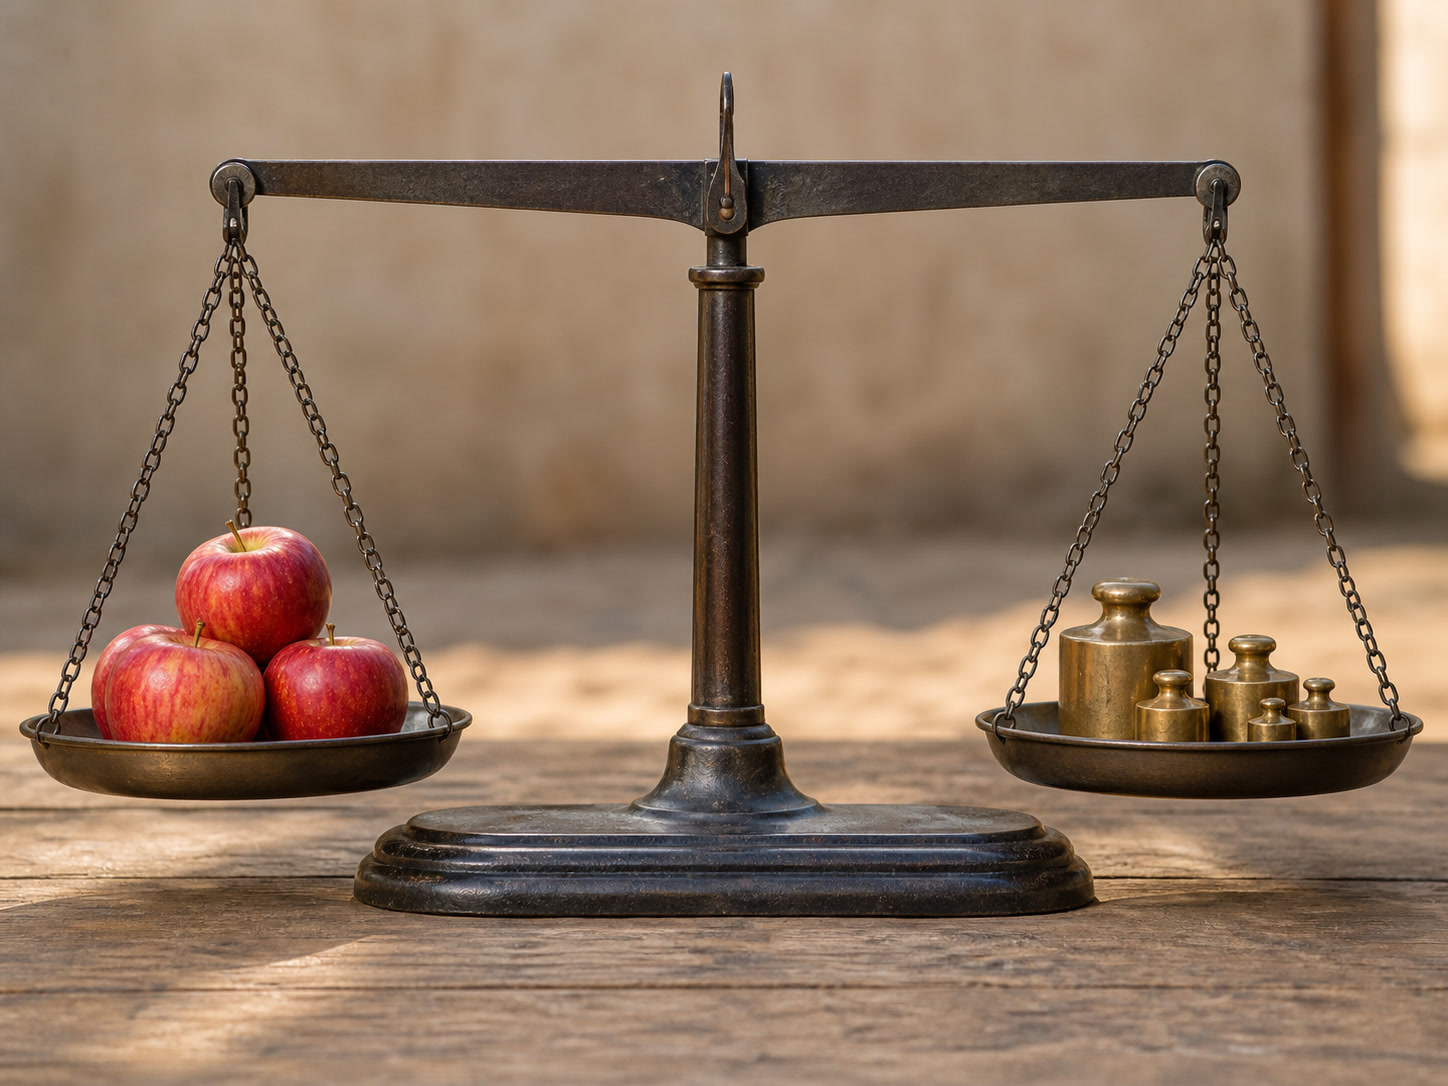
\includegraphics[width=0.52\linewidth]{images/book1/ai/g3-mass-balance-scale.jpg}

{\small Sebuah \omterm{def:g3:levers-and-scales:scale}{neraca} menjalankan tugasnya dengan tenang: piringnya mendatar, jadi \omterm{def:g3:measuring-mass:mass}{massa} apelnya sama dengan total anak timbangan kuningannya.}
\end{omfigure}

\begin{example}[Timbangan yang lain]\label{ex:g3:measuring-mass:otherscales}
Timbangan dapur dan timbangan kamar mandi tidak punya piring kedua:
kamu meletakkan bebannya, dan sebuah jarum berputar (atau sebuah angka
menyala) untuk menunjukkan \omterm{def:g3:measuring-mass:mass}{massanya} langsung. Di dalamnya, sebuah
pegas yang tertekan melakukan perbandingannya untukmu. Praktis dan
cepat --- tetapi \omterm{def:g3:levers-and-scales:scale}{neraca} dua piring yang tua tidak menyembunyikan mesin
apa pun: hanya aturan \omterm{def:g3:levers-and-scales:lever}{tuas} yang sudah kamu pahami.
\end{example}

\begin{example}[Membaca pasar]\label{ex:g3:measuring-mass:market}
``Apel sekilogram'' berarti: apel sampai \omterm{def:g3:levers-and-scales:scale}{neracanya} seimbang dengan
balok \qty{1}{kg} --- kira-kira $6$ atau $7$ buah apel. Tepung dijual
dalam kantong \qty{1}{kg}, batang cokelat sering \qty{100}{g}, sepucuk
surat memerlukan kira-kira \qty{20}{g} kertas, dan aturan tukang pos
``di bawah \qty{20}{g}, satu perangko'' adalah aturan \omterm{def:g3:measuring-mass:mass}{massa}.
\end{example}

\section{Massa mengikuti zatnya}

\begin{proposition}[Zat sama, massa sama]\label{prop:g3:measuring-mass:conserved}
Mengubah \emph{bentuk} sebuah benda tidak mengubah \omterm{def:g3:measuring-mass:mass}{massanya}. Gulunglah
sebola adonan menjadi ular, pipihkan menjadi panekuk, atau potonglah
menjadi empat lalu timbang semua potongannya bersama-sama: \omterm{def:g3:levers-and-scales:scale}{neracanya}
melaporkan \omterm{def:g3:measuring-mass:mass}{massa} yang sama setiap kali. \omterm{def:g3:measuring-mass:mass}{Massa} menghitung zatnya ---
dan memipihkan, menggulung, serta memotong tidak menambah zat maupun
menguranginya.
\end{proposition}

\begin{omfigure}
\begin{tikzpicture}[scale=0.85]
  \draw[thick, omDef!70!black, fill=omDef, fill opacity=0.5]
    (1.3,1.0) circle (0.55);
  \node[below, font=\small, align=center] at (1.3,0.15)
    {sebola adonan:\\\qty{300}{g}};
  \draw[thick, omDef!70!black, fill=omDef, fill opacity=0.5]
    (6.2,0.85) ellipse (1.5 and 0.28);
  \node[below, font=\small, align=center] at (6.2,0.15)
    {digulung jadi ular:\\\qty{300}{g}};
  \draw[thick, omDef!70!black, fill=omDef, fill opacity=0.5]
    (9.55,0.75) circle (0.3);
  \draw[thick, omDef!70!black, fill=omDef, fill opacity=0.5]
    (10.28,0.75) circle (0.3);
  \draw[thick, omDef!70!black, fill=omDef, fill opacity=0.5]
    (9.72,1.32) circle (0.28);
  \draw[thick, omDef!70!black, fill=omDef, fill opacity=0.5]
    (10.4,1.32) circle (0.28);
  \node[below, font=\small, align=center] at (10.0,0.15)
    {empat potong bersama:\\\qty{300}{g}};
\end{tikzpicture}

{\small Satu gumpal adonan, tiga bentuk --- dan satu \omterm{def:g3:measuring-mass:mass}{massa}. \omterm{def:g3:levers-and-scales:scale}{Neracanya}
tidak pernah tertipu oleh perubahan bentuk.}
\end{omfigure}

\begin{remark}[Neraca mengabaikan penampilan]\label{rem:g3:measuring-mass:appearances}
Inilah kekuatan tenang dari \omterm{def:g2:measuring-length:measure}{mengukur}: mata menilai panekuk yang pipih
``lebih besar'' daripada bola asalnya, dan bantal yang mengembang
``lebih berat'' daripada sebuah batu --- tetapi \omterm{def:g3:levers-and-scales:scale}{neraca}, seperti
\omterm{def:g3:temperature-thermometers:temperature}{termometer} dan penggaris sebelumnya, melaporkan zatnya dan tidak lebih
dari itu. Satu demi satu, alat kita menggantikan ``tampaknya'' dengan
``memang begitu''.
\end{remark}

\section{Latihan}

\begin{exercise}[$\star$]\label{exo:g3:measuring-mass:1}
Apa yang dinyatakan \omterm{def:g3:measuring-mass:mass}{massa} sebuah benda? Dua \omterm{def:g2:measuring-length:measure}{satuan} apa yang
\omterm{def:g2:measuring-length:measure}{mengukurnya}, dan berapa \omterm{def:g3:measuring-mass:units}{gram} yang membentuk satu \omterm{def:g3:measuring-mass:units}{kilogram}?
\end{exercise}

\begin{exercise}[$\star$]\label{exo:g3:measuring-mass:2}
Pilihlah \omterm{def:g3:measuring-mass:mass}{massa} yang lebih masuk akal: penjepit kertas --- \qty{1}{g}
atau \qty{1}{kg}? Sebuah apel --- \qty{150}{g} atau \qty{15}{kg}?
Sekarton susu --- \qty{1}{g} atau \qty{1}{kg}? Seekor kucing ---
\qty{4}{kg} atau \qty{400}{kg}?
\end{exercise}

\begin{exercise}[$\star$]\label{exo:g3:measuring-mass:3}
Kedua piring mendatar ketika sebuah labu berhadapan dengan satu balok
\qty{500}{g} dan dua balok \qty{200}{g}. Berapa \omterm{def:g3:measuring-mass:mass}{massa} labu itu?
\end{exercise}

\begin{exercise}[$\star$]\label{exo:g3:measuring-mass:4}
Mengapa \omterm{def:g3:levers-and-scales:scale}{neraca} kosong harus tergantung mendatar sebelum penimbangan
apa pun? (Ingat pedagang yang curang.)
\end{exercise}

\begin{exercise}[$\star$]\label{exo:g3:measuring-mass:5}
Bola pantai jauh lebih besar daripada sekaleng sup, namun kalengnya
yang menekan piringnya turun. Jelaskan dengan
\cref{ex:g3:measuring-mass:bignotcheavy}.
\end{exercise}

\begin{exercise}[$\star$]\label{exo:g3:measuring-mass:6}
Ada berapa \omterm{def:g3:measuring-mass:units}{gram} dalam \qty{2}{kg}? Dalam setengah \omterm{def:g3:measuring-mass:units}{kilogram}? Mana yang
lebih banyak: \qty{1200}{g} atau \qty{1}{kg}?
\end{exercise}

\begin{exercise}[$\star$]\label{exo:g3:measuring-mass:7}
Sebatang cokelat \qty{100}{g} dipatahkan menjadi semua kotak kecilnya,
lalu setiap kotaknya diletakkan di timbangan bersama-sama. \omterm{def:g3:measuring-mass:mass}{Massa}
berapa yang ditunjukkan timbangan itu, dan hukum mana yang
mengatakannya?
\end{exercise}

\begin{exercise}[$\star$]\label{exo:g3:measuring-mass:8}
Timbangan dapur dan \omterm{def:g3:levers-and-scales:scale}{neraca} dua piring sama-sama menimbang sekantong
tepung. Apa yang dipakai masing-masingnya untuk membandingkan --- dan
yang mana yang bekerja dengan aturan yang kamu pelajari tiga bab lalu?
\end{exercise}

\begin{exercise}[$\star$]\label{exo:g3:measuring-mass:9}
Tukang roti memerlukan \qty{800}{g} tepung dan punya balok
\qty{500}{g}, \qty{200}{g}, \qty{200}{g}, \qty{100}{g}, dan
\qty{50}{g}. Carilah dua cara berbeda untuk menimbang tepat
\qty{800}{g} --- dengan mengetahui bahwa balok boleh diletakkan di
\emph{piring mana pun}.
\end{exercise}

\begin{exercise}[$\star\star$]\label{exo:g3:measuring-mass:10}
Nina menimbang sebuah jeruk utuh: \qty{200}{g}. Ia mengupasnya lalu
menimbang jeruk kupasannya saja: \qty{160}{g}. Apakah
\cref{prop:g3:measuring-mass:conserved} gagal? Di mana \omterm{def:g3:measuring-mass:units}{gram} yang
hilang itu, dan bagaimana Nina dapat membuktikannya dengan satu
penimbangan lagi?
\end{exercise}

\begin{exercise}[$\star\star$]\label{exo:g3:measuring-mass:11}
Sebuah teka-teki, yang sekarang mudah bagimu: mana yang \omterm{def:g3:measuring-mass:mass}{massanya} lebih
besar, sekilogram bulu atau sekilogram besi? Dan mana yang memakan
lebih banyak ruang? Jelaskan mengapa begitu banyak orang menjawab
pertanyaan pertama dengan keliru.
\end{exercise}
